
\section{Duality for conic and semidefinite optimization}

\label{conic:optimization}

This chapter is a preparation to describing interior-point methods for SDP. Interior-point methods for SDP rely on SDP duality. Since SDP duality is a special case of conic duality, we start with the conic duality and then specialize it to the SDP case.  

The chapter was motivated by various literature sources including \cite{Laurent:Vallentin:2012} and \cite[Chapter~4]{Gaertner:Matousek:2012}. When discussing general conic programming duality, we'll work in the space $\R^n$ with $n \in \N$. We'll use the notation 
\[
	H^\le(u,\beta) := \setcond{ x \in \R^n}{ \sprod{u}{x} \le \beta}
\]
for $u \in \R^n$ and $\beta \in \R$. If $u \ne 0$, such $H^\le(u,\beta)$ is a closed half-space. An analogous notation can also be used for the relations $=,\ge,<,>$, giving also notation for hyperplanes and open half-spaces.

\subsection{Every nonlinear problem is a conic problem (in principle)}

\newcommand{\SOC}{\operatorname{SOC}}

A conic problem is a problem of optimizing a linear function $\sprod{c}{x}$ under constraints of the form $b_i - A_i x \in L_i$ for all $i \in [s]$, where $b_1,\ldots,b_s$ are vectors, $A_1,\ldots,A_s$ matrices and $L_1,\ldots,L_s$ are closed convex cones. If $L$ is a closed convex cone, the constraint $x \in L$ is a kind of `generalized non-negativity' and is a special case of the constraint $b - A x \in L$ with $b=0$ and $A = -I$. 

It is clear that LP in any of its forms, say, in the form of optimizing $\sprod{c}{x}$ subject to $A x = b$ and $x \ge 0$ is a conic problem. For this form one can use the cones $\{0\}$ and $\R_+^n$ and write the constraints as $b- A x \in \{0\}$ and $x \in \R_+^n$. So, if we use the non-negative orthant in the definition of conic problem, we end up with a linear problem. 

Are there any other interesting cones around? Yes, there are a few other cones which are good in terms of efficiency and are useful for modeling various situations. Consider for example the facility location problem of minimizing $f(x) := \sum_{i=1}^s \|x- p_i\|$, which is the total sum of distances to given facilities $p_1, \ldots,p_s \in \R^n$. We can write the problem as the problem of minimizing $\sum_{i=1}^s y_j$ for with $y_1,\ldots,y_s \in \R$, $x \in \R^n$ and $y_i \le \|x-p_i\|$ for all $i$. If we define the second order cone $\SOC_n:=\setcond{(x,y)}{y \ge \|x\|}$, then our problem can be written using the conic constraints $(x - p_i,y_i) \in \SOC_n$ for $i \in [s]$. 

A very interesting case of conic programming we need in this course is semidefinite programming, arising from the cones $\cS_+^k$ of psd matrices. 

Conic programming is a special case of convex programming. Interestingly, from the perspective of conic programming, we can pretend as every non-linear problem were convex. Consider, for example, the problem $\inf_{x \in \R^n} f(x)$ of constrained optimization of a polynomial $f \in \R[x]$ in $n$ variables of degree at most $d$. Let $K_{n,d}$ be the closed convex cone of all non-negative polynomials of degree at most $d$ in $n$ variables. Then our problem can be rewritten as $\sup \setcond{y \in \R}{f - y \in K_{n,d}}$. This is a conic problem with the decision variable $y$ and the conic constraint $f - y \in K_{n,d}$ for this unknown. Of course, there is a catch here: our problem did not get simpler by transformation into the conic form. The problem remains as difficult as it was. The complexity of the problem is now hidden in the cone $K_{n,d}$, which is a complicated object (checking if a given polynomial belongs to $K_{n,d}$ is hard). Nevertheless, such conic reformulations \emph{can} help computationally. The approach is to express problems using cones and then try to understand the structure of the underlying cones and exploit it in computations. 


\subsection{Duality operations for convex sets}

With each set $X \subseteq \R^n$ we associate the \emph{polar set}
\[
	X^\circ = \setcond{y \in \R^n}{\sprod{y}{x} \le 1 \ \forall x \in X}
\]
and the \emph{dual cone}
\[
	X^\ast = \setcond{y \in \R^n}{\sprod{y}{x} \ge 0 \ \forall x \in X}
\]
In what follows we will need $X^\ast$, but it is not a bad idea to see $X^\circ$ at least once. The set $X^\circ$ is a closed, convex set containing $0$ and $X^\ast$ is a closed convex cone. The following is a main duality statement for the above duality operations. 
\begin{proposition}
	For every non-empty set $X \subseteq \R^n$, one has
	\begin{align*}
		(X^\circ)^\circ & = \cl(\conv(X \cup \{0\})),
		\\ (X^\ast)^\ast & = \cl(\cone(X)).
	\end{align*}
\end{proposition}
\begin{proof}
	(a): We first `spell out' what $(X^\circ)^\circ$ actually is: 
	\begin{align*}
		& & & x' \in (X^\circ)^\circ 
		\\ &\Leftrightarrow & & 
		\sprod{x'}{y} \le 1 \ \text{for all} \  y \in X^\circ
		\\ &\Leftrightarrow & & \sprod{x'}{y} \le 1 \ \text{for all $y$ with $\sprod{y}{x} \le 1\forall x \in X$}. 
	\end{align*}
	This shows that $(X^\circ)^\circ$ is the intersection of all half-spaces of the form $H_{y,1}^\le$ containing the set $X$. Such subspaces definitely contain $0$. So, we see that $X \cup \{0\} \subseteq (X^\circ)^\circ$ holds. Since polar sets are always closed convex sets, we even get $\cl(\conv(X \cup \{0\}) \subseteq (X^\circ)^\circ$, which is the `easy' inclusion. The converse inclusion relies on separation theorems from the theory of convex sets. 
	
	If a point $x'$ does not belong to $\cl(\conv(X \cup \{0\}))$, there exists a hyperplane separation of this point from our set in the following sense: there exists a vector $u$ and values $\alpha $ and $\beta$ with  $\sprod{u}{x'} \ge \alpha > \beta \ge \sprod{u}{x}$ for all $x \in X \cup \{0\}$. In particular one has $\alpha > \beta \ge 0$. For the vector $v := 2 u / (\alpha + \beta)$ we have $\sprod{v}{x'} > 1$ and $\sprod{v}{x} \le 1$ for all $x \in X \cup \{0\}$. This shows, $x'\not\in H_{v,1}^\le$ and $X \cup \{0\} \subseteq H_{v,1}^\le$. Thus, $x' \not \in (X^\circ)^\circ$.
	

	(b): The proof is analogous to (a). We `spell out' what $(X^\ast)^\ast$ means: 
	\begin{align*}
		&& &x' \in (X^\ast)^\ast
		\\ &\Leftrightarrow & &\sprod{x'}{y} \ge 0 & &\text{für alle} \ y \in X^\ast
		\\ &\Leftrightarrow & & \sprod{x'}{y} \ge 0 & & \text{für alle} \ y \ \text{mit} \ \sprod{y}{x} \ge 0 \ \forall x \in X
	\end{align*}
	
	So $(X^\ast)^\ast$ is the intersection of all half-spaces $H_{y,0}^\ge $ given by a vector $y \ne 0$ that contain $X$ as a subset. Following the same steps as in (a), this shows $\cl(\cone(X)) \subseteq (X^\ast)^\ast$. Conversely: if a point $x'$ is not in $\cl(\conv(X))$, then by separation theorems for convex cones there exists a vector $u$ with $\sprod{u}{x'} < 0$ and $\sprod{u}{x} \ge 0$ for all $x \in \cl(\conv(X))$. That is, $x'$ is not in $H_{u,0}^\ge$, while $H_{u,0}^\ge $ contains $X$ as a subset. This gives $x' \not \in (X^\ast)^\ast$. 
\end{proof}


\subsection{Farkas lemmas in conic optimization}


Farkas lemmas in linear programming involve conditions like $A x \le b$ or $x \ge 0$. Recall that Farkas lemmas provide a certificate for infeasiblity. The template for Farkas lemmas is: a system of conditions is infeasible if and only if there is some data (certificate) that can be used to make the infeasiblity algebraically apparent. For conic optimization, we deal with conic constraints of the forms $b - A x \in K$ and $x \in K$, where $K$ is an arbitrary closed cone (choosing $K$ to be a non-negative orthant we get back the linear programming duality). The duality of linear programming is perfect in the sense that it gives a complete characterization of infeasiblity. For conic-programming duality the situation is quite good, too, but not really perfect. There is a necessary and a sufficient condition for infeasiblity that look very similar but do not quite match. 

In one step of the proof we use the following fact

\begin{exercise}
	Show the following. If $A \in \R^{m \times n}$, where $m,n \in \N$, then the image $\im(A)$ of $A$ and the kernel $\ker(A^\top)$ are related by $\im(A) = \ker(A^\top)^\perp$. 
\end{exercise}

The formula $\im(A) = \ker(A^\top)^\perp$ is one possible way to express the duality of linear algebra. 
 

\begin{theorem}[Farkas-lemma for the system $x \in K, A x =b$]
	\label{thm:farkas:kegel}
	Let $K \subseteq \R^n$ be a closed convex cone, let $A \in \R^{m \times n}$ and $b \in \R^m$. Then implications (1) $\Rightarrow$ (2) $\Rightarrow$ (3) hold for conditions (1), (2) and (3) described as follows: 
	\begin{enumerate}[(1)]
		\item There exists an $y \in \R^m$ with $A^\top y \in K^\ast$ and $\sprod{y}{b} < 0$.
		\item There exists no $x \in K$ with $A x = b$.
		\item There exists $y \in \R^m$ with $A^\top y \in K^\ast$ and $\sprod{y}{b} \le 0$, where $A^\top y$ or $\sprod{y}{b}$ is not $0$.
	\end{enumerate}
	In other words, (1) is a sufficient condition for infeasiblity of the system $x \in K, A x = b$, while (3) is a necessary one.
\end{theorem}
\begin{proof}
	We introduce the notation $X := \setcond{x \in \R^n}{A x = b}$. 
	
	(1) $\Rightarrow$ (2): Assume to the contrary, that there exists an $x \in K \cap X$. Then $\sprod{y}{b } = \sprod{y }{A x} = \sprod{A^\top y}{x} \ge 0$, which contradicts $\sprod{y}{b} < 0$.
	
	(2) $\Rightarrow$ (3): In the degenerate case $X = \emptyset$ we rely on linear algebra. One has $b \not \in \im(A)$. Because of $\im(A)= \ker(A^\top)^\perp$ there exists $y$ with $A^\top y = 0$ and $\sprod{y}{b} \ne 0$. Possibly, replacing $y$ by $-y$, we can assume  $\sprod{y}{b} < 0$. Thus, $y$ is the desired vector. 
	
	In the case $X \ne \emptyset$, we use separation theorems for the sets $K$ and $X$ satisfying $K \cap X = \emptyset$. There exist a vector $u \in \R^n \setminus \{0\}$ and a scalar $\alpha$ with $\sprod{u}{x} \ge \alpha$ for all $x \in K$ and $\sprod{u}{x} \le \alpha$ for all $x \in X$. 
	
	Since $K$ is a cone, the inequality $\sprod{u}{x} \ge \alpha $ for all $x \in K$ implies $\sprod{u}{x} \ge 0$ for all $x \in K$. That is $u \in K^\ast$. For $x=0$ the inequality $\sprod{u}{x}  \ge \alpha$ yields $0 \ge \alpha$. Thus, $\sprod{u}{x} \le \alpha \le 0$ holds for all $x \in X$. The function $x \mapsto \sprod{u}{x}$ is a bounded affine function on the affine space $X$. So, the function is constant on $X$. Then $\sprod{u}{x'} = \sprod{u}{x''}$ for all $x', x'' \in X$. Hence $\sprod{u}{x} =0$ for $X - X = \ker(A)$. Hence $u \in \ker(A)^\perp.$ 
	
	Since $\ker(A)^\perp = \im(A^\top)$, one has $u = A^\top y$ for some $y$. Thus, $\sprod{u}{x} = \sprod{A^\top y}{x} = \sprod{y}{A x} = \sprod{y}{b} \le \alpha \le 0$ for all $x \in X$. The vector $u=A^\top y$ is not  $0$.
\end{proof}



\subsection{Duality of conic optimization problems}
\label{subsec:konische:Dualitaet}

We'll extend the LP-duality corresponding to the case $K=\R_+^n$ to general closed cones $K$. The weak duality extends easily, for the extension of the strong duality we need a kind of assumption that excludes degenerate situations. 

\begin{theorem}
	\label{thm:kon:dualitaet}
	Let $K \subseteq \R^n$ be closed convex cone, let $A \in \R^{m \times n}, b \in \R^m$ and $c \in \R^n$ and consider the following conic problems
	\begin{align}
		\alpha & = \inf \setcond{\sprod{c}{x}}{x \in K, \ Ax -b = 0 } \label{eq:kon:primal}
		\\ \beta & = \sup \setcond{\sprod{y}{b}}{y  \in \R^m, \  c - A^\top y \in K^\ast}. \label{eq:kon:dual}
	\end{align}
	Then the following hold:
	\begin{enumerate}[(a)]
		\item If both \eqref{eq:kon:primal} and \eqref{eq:kon:dual} have feasible solutions, then $\alpha \ge \beta$. 
		\item If \eqref{eq:kon:primal} is unbounded ($\alpha= -\infty$), then \eqref{eq:kon:dual} is infeasible ($\beta = -\infty$)
		\item If \eqref{eq:kon:dual} is unbounded ($\beta=+\infty$), then \eqref{eq:kon:primal} is infeasible ($\alpha = +\infty$). 
		\item If there exists $x' \in \intr(K)$ with $A x' - b = 0$, then one has equality $\alpha = \beta$.
	\end{enumerate}
\end{theorem}
\begin{proof}	
	(a): For every feasible solution $x$ of \eqref{eq:kon:primal} and every feasible solution $y$ of \eqref{eq:kon:dual} one has $\sprod{A x -b }{y} = 0$ because $A x -b  = 0 $. On the other hand, one has $\sprod{c - A^\top y}{x} \ge 0$  by $x\in K$ and $c - A^\top y  \in K^\ast$. Thus, we get
	\[
		\sprod{c}{x} \ge \sprod{A^\top y}{x} = \sprod{A x }{y} = \sprod{b}{y}.
	\]
	
	(b) and (c) follow from (a).
	
	(d):  The existence of $x'$ implies $\alpha < \infty$. In the degenerate case $\alpha = -\infty$, the equality follows from (b). We consider the case $-\infty < \alpha < \infty$. Let $X := \setcond{x \in \R^n}{A x = b}$.
	
	
	Fix an arbitrary $\eps> 0$. By the definition of $\alpha$ there exists no $x$ with $x \in K$, $\sprod{c}{x} = \alpha - \eps$ and $A x  = b$. Application of the implication (2) $\Rightarrow$ (3) of  Theorem~\ref{thm:farkas:kegel} (Farkas-Lemma) to the system
	\begin{align*}
		x & \in K,
		&
		\begin{pmatrix}
			-A 
			\\ 
			c^\top
		\end{pmatrix}
			x
		& = \begin{pmatrix}
			-b
			\\
			\alpha - \eps
		\end{pmatrix}
	\end{align*}
	yields the existence of $y \in \R^m$ and $\mu \in \R$ with $\mu c - A^\top y \in K^\ast$ and $\mu( \alpha - \eps) - \sprod{y}{b} \le 0$, where $\mu c - A^\top y$ or $\mu(\alpha - \eps) - \sprod{y}{b}$ is not $0$. We'll produce a feasible solution of the dual problem out of  $\mu$ and $y$. Since the dual solution will have to be linked to the primal one, we derive the following inequalities:
	\begin{equation}
		\label{eq:maybe:strict}
		\mu \sprod{c}{x'} - \sprod{y}{b} = \mu \sprod{c}{x'} - \sprod{y}{A x'} = \sprod{\underbrace{\mu c - A^\top y}_{\in K^\ast}}{\underbrace{x'}_{\in K}} \ge 0,
	\end{equation}
	So, we get
	\begin{equation}
		\label{eq:at:least:one:is:strict}
		\mu(\alpha - \eps) \le \sprod{y}{b} \le \mu \sprod{c}{x'} 
	\end{equation}
	By the implication (2) $\Rightarrow$ (3) of Theorem~\ref{thm:farkas:kegel} one has $\mu c - A^\top y \ne 0$ or $\mu ( \alpha - \eps) - \sprod{y}{b} < 0$. In the former case, the inequality in \eqref{eq:maybe:strict} is strict, because $x'$ lies in $\intr(K)$. In the latter case the inequality $\mu (\alpha - \eps) < \sprod{y}{b}$ is strict. This yields that at least one of the two inequalities in \eqref{eq:at:least:one:is:strict} is strict. We get $\mu (\alpha - \eps) < \mu \sprod{c}{x'}$. 

	Taking into account that $\sprod{c}{x'} > \alpha - \eps$  holds for all $x \in K \cap X$, we get $\mu > 0$. Now, wlog we can assume $\mu=1$, because we can rescale $y$  to $y/\mu$ and $\mu$ to $\mu/\mu =1$. After this change we get $c - A^\top y \in K^\ast$ and $\sprod{y}{b} \ge \alpha - \eps$. So, for an arbitrary $\eps>0$ we have found a feasible solution of  \eqref{eq:kon:dual}, which satisfies $\sprod{y}{b} \ge \alpha - \eps$. Thus, $\beta \ge \alpha - \eps$ for every $\eps> 0$, and we get the inequality $\beta \ge \alpha$.
\end{proof}

The conic problems \eqref{eq:kon:primal} and \eqref{eq:kon:dual} are called \emph{dual} to each other. The assertions (a)-(c) are called \emph{weak duality}, and the assertion (d) is called \emph{strong duality}. 

\begin{exercise}
	\label{compl:slackness}
	Show that, in the notation of  Theorem~\ref{thm:kon:dualitaet}, the following hold: 
	\begin{enumerate}[(a)]
		\item If $x$ and $y$ are feasible solutions of \eqref{eq:kon:primal} and \eqref{eq:kon:dual}, respectively and $\sprod{c -A^\top y}{x} = 0$ holds, then $x$ and $y$ are optimal for \eqref{eq:kon:primal} and \eqref{eq:kon:dual}, respectively. 
		\item If $\alpha = \beta$ and \eqref{eq:kon:primal} and \eqref{eq:kon:dual} have optimal solutions $x^\ast$ and $y^\ast$, respectively, then $\sprod{c - A^\top y^\ast}{x^\ast} =0$ holds. 
	\end{enumerate}
\end{exercise}
\begin{solution}
	To get both assertions, just look at the derivation of the weak duality
	\[
		\sprod{b}{y} = \sprod{A x}{y} = \sprod{x}{A^\top y} \le \sprod{x}{c}.
	\]
\end{solution}

\subsection{Duality for more general formulations}

In conic optimization, similarly to linear programming, we can formulate duality for different or more general formulations. 

We'll need the following simple observation. 

\begin{exercise}
	\label{dual:of:product}
	Let $n_1,\ldots,n_t \in \N$ and $t \in \N$. Consider, for every $i \in [t]$, the set $X_i \subseteq \R^{n_i}$ with $0 \in X_i$. Then 
	\[
		(X_1 \times \ldots \times X_t)^\ast = X_1^\ast \times \ldots \times X_t^\ast. 
	\]
\end{exercise}
\begin{solution} 
	$(y_1,\ldots,y_t) \in (X_1 \times \ldots \times X_t)^\ast$ means $\sprod{(y_1,\ldots,y_t)}{(x_1,\ldots,x_t)} \ge 0$ for all $(x_1,\ldots,x_t) \in X_1 \times \ldots \times X_t$. Plugging in $0$ for all  $x_i$ but one, we get $\sprod{y_i}{x_i} \ge 0$ for all $i \in [t]$ and $x_i \in X_i$. This shows $y_i \in X_i^\ast$ for all $i \in [k]$. The converse inclusion $X_1^\ast \times \ldots \times X_t^\ast \subseteq (X_1 \times \ldots \times X_t)^\ast$ also follows directly: a vector $(y_1,\ldots,y_t)$ belonging to the left hand side satisfies  $\sprod{y_i}{x_i} \ge 0$ for all $i \in [t]$ and all $x_i \in X_i$. This yields $(y_1,\ldots,y_t) \in (X_1 \times \ldots \times X_t)^\ast$.
\end{solution}

\begin{exercise}
	Show the following. Let $m, n \in \N$, let $K \subseteq \R^n$ and $L \subseteq \R^m$ be closed convex cones and let $A \in \R^{m \times n}, c \in \R^n$ and $b \in \R^m$. Consider the problems
	\begin{equation}
		\label{eq:primal:K:L}
	\alpha := \inf \setcond{ \sprod{c}{x} }{x \in K, \ A x - b \in L}
	\end{equation}
	and
	\begin{equation}
		\label{eq:dual:K:L}
	\beta := \sup \setcond{ \sprod{y}{b}}{y \in L^\ast, \ c - A^\top y \in K^\ast}.
	\end{equation}
	Then the following hold:
	\begin{enumerate}[(a)]
		\item The problems satisfy weak duality. 
		\item If there exists an $x'$ with $x' \in \intr(K)$ and $A x - b \in \intr(L)$, then strong duality holds.
		\item If there exists an $y'$ with $y' \in \intr(L^\ast)$ and $c - A^\top y \in \intr(K^\ast)$, then strong duality holds.
	\end{enumerate}
\end{exercise}
\begin{solution} 
	\emph{(a):} We reformulate the minimization problem as follows:
	\begin{align*}
		\alpha & = \inf \setcond{ \sprod{c}{x} }{ (x,u) \in K \times L, \ A x - u = b}
		\\ & = \inf \setcond{ \sprod{\begin{pmatrix} c \\ 0 \end{pmatrix} }{ \begin{pmatrix} x \\ u \end{pmatrix} } }{ (x,u) \in K \times L, \ \begin{pmatrix} A & -I \end{pmatrix} \begin{pmatrix} x \\ u \end{pmatrix} = b}
	\end{align*}
	Application of Theorem~\ref{thm:kon:dualitaet} yields the dual problem
	\[
		\sup \setcond{\sprod{y}{b}}{ \begin{pmatrix}c\\ 0 \end{pmatrix} - \begin{pmatrix} A^\top \\ - I \end{pmatrix} y  \in (K \times L)^\ast}.
	\]
	Application of Exercise~\ref{dual:of:product} yields $(K \times L)^\ast = K^\ast \times L^\ast$.
	 So, the latter problem can be reformulated as \eqref{eq:dual:K:L}.
	 
	\emph{(b):} From the proof of (a) and in view of  Theorem~\ref{thm:kon:dualitaet}, one can see that the strong duality holds whenever there exists $(x',u') \in \intr(K \times L) = \intr(K) \times \intr(L)$ with $Ax' - u' =b$.

	\emph{(c):} We reformulate \eqref{eq:dual:K:L} as a minimization problem:
	\[
		-\beta = \inf \setcond{\sprod{y}{-b}}{y \in L^\ast, \ (-A^\top) y - (-c) \in K^\ast}.
	\]
	Application of (b) to this minimization problem yields
	\[
		- \beta = \sup \setcond{\sprod{x}{-c}}{x \in (K^\ast)^\ast,  \ (-b) - ((-A)^\top)^\top x  \in (L^\ast)^\ast }.
	\]
	In view of $(K^\ast)^\ast = K$ and $(L^\ast)^\ast = L$ we get
	\[
		- \beta = \sup \setcond{ - \sprod{c}{x} }{x \in K, \ A x - b \in L} = - \alpha.
	\]
	So, $\alpha = \beta$. 
\end{solution}

\begin{remark}
	Now, having deduced the more general form of duality, we can `update'  Theorem~\ref{thm:kon:dualitaet} that we had formulated before. In fact, there exists another case of strong duality for problems discussed in Theorem~\ref{thm:kon:dualitaet}, namely, when there exists $y' \in \R^m$ with $c - A^\top y'\in \intr(K^\ast)$. Observe, that the whole space $\R^m$ is a convex cone whose dual cone is $(\R^m)^\ast = \{0\}$. Thus, what we do is just use the corollary for $L=\R^n$. 
\end{remark} 

We conclude this section by formulating a very general form of conic duality with an arbitrary number of conic constraints. 

\begin{exercise}
	\label{cor:K:L:dual}
	Show the following. Let $t, s \in \N$ and consider the problems
	\[
		\alpha  = \inf \setcond{\sum_{i=1}^t \sprod{c_i}{x_i} }{x_i \in K_i \ \forall i \in [k], \ \sum_{j=1}^t A_{i,j} x_j - b_i \in L_i \ \forall i \in [s]}
	\]
	and
	\[
		\beta = \sup \setcond{ \sum_{i=1}^s \sprod{b_i}{y_i} }{y_i \in L_i^\ast \ \forall i \in [s], \ c_i - \sum_{j=1}^s A_{j,i}^\top y_j  \in K_i^\ast \ \forall i \in [t]}
	\]
	based on closed convex cones $K_1,\ldots,K_t, L_1,\ldots,L_s$, Matrices $A_{i,j}$ with $i \in [s], j \in [t]$ and vectors $c_1,\ldots,c_t,b_1,\ldots,b_s$. Then: 
	\begin{enumerate}[(a)]
		\item The weak duality holds for this pair of problems.
		\item If the minimization problem has solution $(x_1',\ldots,x_t')$ with $x_i' \in \intr(K_i)$ for all $i \in [t]$ and $\sum_{j=1}^t A_{i,j} x_j' - b_i \in \intr(L_i)$ for all $i \in [s]$, then the strong duality holds.
		\item If the maximization problem has a solution $(y_1',\ldots,y_s')$ with $y_i \in \intr(L_i^\ast)$ for all $i \in [s]$ and $c_i - \sum_{j=1}^s A_{j,i}^\top y_j \in \intr(K_i^\ast)$, then the strong duality holds.
	\end{enumerate}
\end{exercise}
\begin{solution}
	Let $x=(x_1,\ldots,x_k)$. Let $c=(c_1,\ldots,c_t)$, $b=(b_1,\ldots,b_t)$ and let $A$ be the matrix with blocks $A_{i,j}$. Then our problems can be formulated concisely as
	\[
		\inf \setcond{\sprod{c}{x}}{x \in K_1 \times \ldots \times K_t,  \ A x - b \in L_1 \times \ldots \times L_s }
	\]
	and
	\[
		\beta = \sup \setcond{\sprod{b}{y}}{y \in L_1^\ast \times \ldots \times L_t^\ast, \ c- A^\top y \in K_1^\ast \times \ldots \times K_t^\ast}
	\]
	The assertions now follow from Exercise~\ref{cor:K:L:dual} and Exercise~\ref{dual:of:product}.
\end{solution}


\subsection{Semidefinite optimization}

Semidefinite optimization was introduced in Section~\ref{SOS:and:sdp}. Here, we are able to describe semidefinite problems concisely as a special conic problem. We work with linear spaces $\cS^k$ and with the cones $\cS_+^k$ in these spaces. For being able to write systems of linear inequalities concisely it is nice to have a scalar product fixed in $\cS^k$. The space $\cS^k$ is a subspace of $\R^{k \times k}$ (all $k \times k$ matrices, not necessarily symmetric), and in $\cS^k$ one can borrow a scalar product from $\R^{k \times k}$. For $\R^{k \times k}$, a very natural scalar product is the standard one: we can think of $\R^{k \times k}$ as a vector with $k^2$ components and define the scalar product as the standard scalar product of such vectors. It turns out that this scalar product can be expressed nicely using the trace operation: It is straightforward to check that for $A = (a_{ij}), B= (b_{ij}) \in \R^{k \times k}$, one has 
\[
	\sprod{A}{B}:= \sum_{i,j} a_{ij} b_{ij} = \tr(A B^\top) = \tr(A^\top B).
\] Of course, if our matrices are symmetric we need not transpose so that we get the formula $\sprod{A}{B} = \tr(A B)$ for $A, B \in \cS^k$. 


Geometrically, SDP can be formulated as an optimization of a linear function over an affine slice of $\cS_+^k$. That is, one optimizes a linear objective over $\cS_+^k \cap H$, where $H \subseteq \cS^k$ is an affine space. There are two ways to represent $H \cap \cS_+^k$ algebraically: one can parameterize $H$ or one can describe $H$ by a system of linear inequalities. As a consequence, there are the following two basic formulations of SDP.

If we use equalities to describe $H$, we get a formulation
\[
	\inf \setcond{ \sprod{C}{X} }{ X \in \cS_+^k, \ \sprod{A_i}{X} = b_i \ \forall i \in [m]},
\]
where $C, A_1,\ldots,A_m \in \cS^k$ and $b_1,\ldots,b_m \in \R$. If we parameterize $H$ we end up with 

\[
	\inf \setcond{ \sprod{c}{x}}{x \in \R^n, A(x) \in \cS_+^k},
\]
with $c \in \R^n$, where $A : \R^n \to \cS^k$ is affine map, meaning  $A(x_1,\ldots,x_n) = A_0 + A_1 x_1 + \cdots + A_n x_n$ for some $A_0,\ldots,A_n \in \cS^k$. The condition $A(x) \in \cS_+^k$ is a \emph{linear matrix inequality} for $x$, which we have already seen in Section~\ref{SOS:and:sdp}
(abbreviated as LMI). The expression $A(x)$ can be viewed as an affine function in $x$ with matrix coefficients or as symmetric matrices whose entries are affine functions in $x$.

LMIs are generalizations of linear inequalities (if the off-diagonal entries of $A(x)$ are identically equal to zero, we merely have a system of $k$ linear inequalities). 
Here is a picture illustrating the geometry of sets described by LMIs (such sets are called spectrahedra):
\begin{center}
	\begin{tikzpicture}[]
	\pgftext{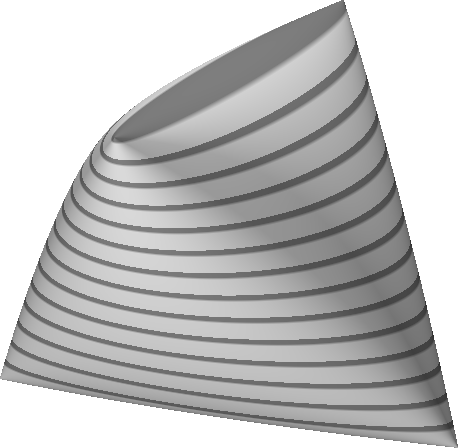
\includegraphics[width=150pt]{spectrahedron}} at (0pt,0pt);
	\node[align=left] at (7,0) {\(
		\begin{pmatrix} 1 & x_1 & x_2 \\ x_1 & 1 & x_3 \\ x_2 & x_3 & 1
		\end{pmatrix} \ \text{psd}
		\)
	};
	\end{tikzpicture}
\end{center}

The first thing we wish to do is discussing duality for SDP. We would like to use the results from the previous sections. While in the previous sections we worked with the duality with respect to the standard scalar product in $\R^n$, it is clear that the duality could have been introduced with respect to any scalar product and the results would still be the same. So, we can introduce the dual cone $(\cS_+^k)^\ast$ in the space $\cS^k$ just by the same formula that we used to introduce dual cones in $\R^n$.

It turns out that $\cS_+^k$ is self-dual.

\begin{exercise}
	For every $k \in \N$ one has $(\cS_+^k)^\ast = \cS_+^k$ (the cone $\cS_+^k$ is self-dual). 
\end{exercise}
\begin{solution} 
	For $A \in \cS^k$ the equality says that the condition $A \in \cS_+^k$ is equivalent to $\sprod{A}{B} \ge 0 \ \forall B \in \cS_+^k$. We check this equivalence.
	
	If $A \in \cS_+^k$, then  $\sprod{A x}{x} \ge 0$ holds for all $x$. The latter can be turned into the form $\sprod{A}{x x^\top} \ge 0$. Note that $x x^\top$ is a symmetric (psd) matrix of rank $1$ (for $x \ne 0$). The cone $\cS^k_+$ is the conic hull of all such matrices (see Exercise~\ref{sdp:sum:rank:1}). So, we get $\sprod{A}{B} \ge 0$ for all $B \in \cS_+^k$. Conversely: if $\sprod{A}{B} \ge 0$ holds for every $B \in \cS_+^k$, then choosing $B = x x^\top$, we get $\sprod{A}{x x^\top} \ge 0$ for all $x \in \R^n$. This gives $\sprod{A x}{x } \ge 0$ for all $x$ and shows $A \in \cS_+^k$. 
\end{solution}

\begin{exercise}
	Formulate the problem of computing the largest eigenvalue of a symmetric matrix as an SDP. 
\end{exercise}
\begin{solution}
	For $A \in \cS^k$ consider the matrix $t I - A$. It is easy to see that $\lambda$ is an eigenvalue of $A$ if and only if $t-\lambda$ is an eigenvalue of $t I - A$. A matrix $A$ is psd if and only if all its eigenvalues are non-negative. So, we arrive at the SDP
\begin{align*}
	\min \setcond{t \in \R}{ t I - A \in \cS_+^k}
\end{align*}
with one decision variable $t \in \R$.
This is an SDP in one unknown $t \in \R$. 
In the same way, we can see that computation of the spectral norm of a symmetric matrix is again an SDP (in one unknown).
\end{solution}

\begin{remark}
	Many researches are very excited about SDP. Why? It has turned out that a large number of problems can be formulated (exactly or approximately) as SDP. In particular, we have seen that polynomial problems can be formulated approximately as SDPs. Apart from that, SDPs arise in control theory, combinatorial optimization, statistics, probability etc. Yet another reasons for excitement is that SDP leads to interesting mathematical problems involving algebra, convexity and algorithms. 
\end{remark}

\subsection{Duality for SDP}

Using the previous section and conic duality, we can derive duality for SDPs. For duality in the space $\R^n$ we used the standard scalar product in $\R^n$, and the matrix $A$ (of the left hand side of the underlying system of constraints) in the primal problem has been turned to the transposed matrix $A^\top$ in the dual problem. Now, we work in $\cS^k$, which is a different Euclidean space, and so instead of using $A^\top$ we need to use an abstract analogue of it. The abstract transpose is called the adjoint operator. Actually, the adjoint operator is just another way of writing transpose (it's not more general in its essence, it's just a more general way of writing things down, that does not rely too much on the components). Let me shortly recall how this works (this material is typically presented in linear algebra). We've got two finite-dimensional Euclidean spaces $V$ and $W$ over $\R$. The spaces have scalar products  $\sprod{\dotvar}{\dotvar}_V$ and $\sprod{\dotvar}{\dotvar}_W$ (frequently, one would just omit the subscript, as it is usually clear which of the scalar products is meant). 

Consider a linear map $A : V \to W$ and a vector $b \in W$. With this data we can define an `abstract' linear system $A(x) = b$ in the unknown $x \in V$. An analogue of transpose matrix is the so-called \emph{adjoint operator} or \emph{adjoint map} $A^\ast : W \to V$, defined as the unique linear map satisfying $\sprod{A(x)}{y}_W = \sprod{x}{A^\ast(y)}_V$. 

In this abstract setting the dual pair of conic programs looks as follows

\[
	\inf \setcond{ \sprod{c}{x}}{ x \in K, \ A (x) - b \in L}
\]
and
\[
	\sup \setcond{ \sprod{y}{b}}{y \in L^\ast, \ c - A^\ast (y) \in K^\ast}
\]
where $K$ is a closed convex cone in $V$ and $L$ a closed convex cone in $W$. 



\newcommand{\cA}{\mathcal{A}}
We just need to specify what we get in the case of SDPs in the above formulas. For example, let's determine the dual of the SDP in the form
\[
	\inf \setcond{ \sprod{c}{x}}{ x_1 A_1 + \ldots + x_n A_n - B \in \cS_+^k}
\]

We can write it as 
\[
	\inf \setcond{ \sprod{c}{x}}{x \in \R^n, A(x) - B \in \cS_+^k}
\]
where $A : \R^n \to \cS^k$ is the linear map $A(x) = A_1 x_1 + \cdots + A_n x_n$. To get the dual we need to determine $A^\ast : \cS^k \to \R^n$. Just use the equality that defines the adjoint map:
\[
	\sprod{A(x)}{Y} = \sprod{x}{A^\ast(Y)} \qquad \forall x \in \R^n \ \forall Y \in \cS^k.
\]
This can be spelled out as
\[
	\sprod{A_1 x_1 + \ldots + A_n x_n}{Y} = \sprod{(x_1,\ldots,x_n)}{A^\ast(Y)} \qquad \forall x_1,\ldots,x_n \in \R \ \forall Y \in \cS^k.
\]
Comparing coefficients for $x_1,\ldots,x_n$ gives the formula 
\[
	A^\ast(Y) = ( \sprod{A_1}{Y},\ldots, \sprod{A_n}{Y})
\]
for the adjoint map.

Consequently, our dual problem is 
\[
	\sup \setcond{ \sprod{B}{Y}}{Y \in \cS_+^k, \ c_i = \sprod{A_i}{Y} \ \forall i \in [n]}
\]

\begin{remark}
	If you know the mnemonic rules to get a dual LP, you see that these rules carry over to the case of SDP in some very natural way. The mnemonic rule is about what corresponds to what in the primal-dual pair:
	\begin{itemize}
		\item variables $\leftrightarrow$ constraints
		\item unconstrained variables$\leftrightarrow$ equality constraints
		\item non-negative variables $\leftrightarrow$ inequality constraints;
		\item right hand sides $\leftrightarrow$ coefficients of the objective functions. 
	\end{itemize}
	We see that the rule remains valid for SDP.
	Our primal problem had $x_1,\ldots,x_n$ unconstrained real variables and one SDP constraint. The sdp constraint generates a psd-constrained variable $Y$ in the dual. The $n$ variables $x_1,\ldots,x_n$ generate the $n$ equality constraints in the dual. Note that our primal/dual pair of SDP illustrates the following: 
	\begin{itemize}
		\item real variables $\leftrightarrow$ LP constraints ($=$ linear (in)equalities)
		\item matrix variables $\leftrightarrow$ SDP constraints ($=$ LMIs).
	\end{itemize}
\end{remark}

\subsection{SDP duality applied to polynomial optimization}

Let's now apply the SDP duality to the SDP problem we derived in Section~\ref{SOS:and:sdp}. Let me remind what we did. We wanted to solve the global POP 
\begin{equation}
	\label{global:pop}
	\inf \setcond{f(x)}{ x \in \R^n },
\end{equation}
where $f(X)= \sum_{\alpha \in E^n_{2d}} c_\alpha X^\alpha \in \R[X]=\R[X_1,\ldots,X_n]$. We introduce a formal dual problem $\sup \setcond{y}{f - y \ge 0 \ \text{on} \  \R^n}$ (the problem to find the lower bounds) and then replaced this problem by the simpler problem
\[
	\sup \setcond{y \in \R}{ f - y \quad \text{sos}}, 
\]
which turned out to be the SDP
\[
	\sup \setcond{y \in \R}{ y + m(X)^\top Z m(X) = f(X), \ Z \ \text{psd} }
\]
where $m(X)= (X^\alpha)_{\alpha \in E^n_d}$ is the vector of monomials of degree at most $d$. So, the above problem is a problem with decision variables $y$ and $Z$. To dualize the problem, we write the equality constraint $y + m(X)^\top Z m(X) = f(X)$ in coordinate form. Let $Z=(z_{\alpha,\beta})_{\alpha,\beta \in E^n_d}$. Then the equality $y + m(X)^\top Z m(X)= f(X)$ is 
\[
	y + \sum_{\alpha,\beta \in E^n_d} z_{\alpha,\beta} X^{\alpha+\beta} = \sum_{\gamma \in E^n_{2d}} c_\gamma X^\gamma.
\]
Comparing coefficients we get
\[
	y + z_{0,0} = c_0
\] 
and 
\begin{align*}
	\sum_{\alpha,\beta \in E^n_d : \ \alpha + \beta =\gamma} z_{\alpha,\beta} &=  c_\gamma & & \forall \gamma \in E^n_{2 d} \setminus \{0\}
\end{align*}

The latter can be written as equalities
\begin{align*}
	y + \sprod{A_0}{Z}  = c_0
\end{align*}
and
\begin{align*}
	\sprod{A_\gamma}{Z} &= c_\gamma & &\forall \gamma \in E^n_{2d} \setminus \{0\},
\end{align*}
where
\begin{align*}
	A_\gamma &:= (\delta_{\alpha+\beta,\gamma})_{\alpha,\beta \in E^n_d} & & \forall \gamma \in E^n_{2d}
\end{align*}
are symmetric matrices (we use the Kronecker delta notation: $\delta_{s,t}=1$ if $s=t$ and $\delta_{s,t}=0$ otherwise). Thus, our problem can now be written as 

\begin{equation}
	\label{global:sos:rel:with:equalities}
	\sup \setcond{y \in \R}{ Z \ \text{psd}, \ y+ \sprod{Z}{A_0} = c_0, \ \sprod{A_\gamma}{Z} = c_\gamma \ \text{for \ all} \ \gamma \in E^n_{2d} \setminus \{0\}}.
\end{equation}

Problem \eqref{global:sos:rel:with:equalities} can be dualized according to the principles we've discussed in previous sections.  The psd matrix variable $Z$ yields a psd constraint. The real variable $y$ yields a linear equality. Each linear equality constraint for $\gamma \in E_{2d}^n$ yields a real variable, which we denote by $v_\gamma$.


The dual is the following problem

\[
	\inf \setcond{ \sum_{\gamma \in E^n_{2d} } v_\gamma c_\gamma }{v_\gamma \in \R \ \forall \gamma \in E^n_{2d}, \ \sum_{\gamma \in E^n_{2d}} v_\gamma A_\gamma \ \text{psd}, \ v_0 = 1}
\]

Taking into account how $A_\gamma$ were defined we see that 
\[
	\sum_{\gamma \in E^n_{2d}} v_\gamma A_\gamma = \Biggl( \sum_{\gamma \in E^n_{2d}} v_\gamma \delta_{\alpha + \beta,\gamma} \Biggr)_{\alpha, \beta \in E^n_d} = \Bigl( v_{\alpha+ \beta} \Bigr)_{\alpha, \beta \in E^n_d}.
\]

So, the dual SDP gets the form

\[
	\inf \setcond{ \sum_{\gamma \in E^n_{2d}} v_\gamma c_\gamma }{v_\gamma \in \R \ \forall \gamma, \ \Biggl(v_{\alpha+\beta}\Biggr)_{\alpha, \beta \in E^n_d} \ \text{psd}, \ v_0 = 1}.
\]

\begin{remark}
The problem \eqref{global:sos:rel:with:equalities} was established to derive lower bounds on \eqref{global:pop}, but \eqref{global:sos:rel:with:equalities} does not directly suggest any choice of $x \in \R^n$ that may be good. It turns out that an $x$ can be chosen from the dual problem. It is known that, under certain assumptions, $x=(x_1,\ldots,x_n)$ with 
\begin{align*}
 x_1 & := v_{(1,0,\ldots,0)}, & x_2 & := v_{(0,1,0\ldots,0)}, & & \ldots & x_n & := v_{(0,\ldots,0,1)}
\end{align*}
is a good choice (see works of Marshall, Schweighofer, Lasserre, Laurent et al.). 
\end{remark}

\subsection{Truncated moment problem}

There is another way to arrive at the dual problem we've seen in the last section. 

We show how the approach works for the unconstrained POP only, with the constrained case being similar.

\begin{equation}
	\label{our:inf:problem}
	\inf \setcond{f(x) }{x \in \R^n}
\end{equation}
with $f \in \R[X]=R[X_1,\ldots,X_n]$. Let $c = (c_\alpha)_{\alpha \in E_{2d}^n}$ be the vector of coefficients of $f$ and $m(X) = \setcond{ X^\alpha }{\alpha \in E_{2d}^n}$ the vector of all respective monomials. Then the problem can be written as 
\begin{equation}
	\inf \setcond{ \sprod{c}{m(x)} }{x \in \R^n}.
\end{equation}
This can be viewed as a linear optimization over the set $m(\R^n):=\setcond{m(x)}{x \in \R^n}$. Thus, the problem is
\begin{equation}
	\inf \setcond{\sprod{c}{v}}{v \in m(\R^n)}.
\end{equation}
If we enlarge $m(\R^n)$ to $\conv(m(\R^n))$ or even to $\cl(\conv(m(\R^n)))$, the problem remains the same. This way we arrive at 
\begin{equation}
	\label{lin:probl:on:M}
	\inf \setcond{\sprod{c}{v}}{ v \in M_{n,2d}}.
\end{equation}
In general, $M_{n,2d}$ is hard to describe, but at least we can relax it to a set that we can describe with SDP. By Caratheodory's theorem, every element of $v \in \conv(m(\R^n))$ is the convex combination of at most $\dim(m(\R^n))+1$ points of $m(\R^n)$. This convex combination can be written as integration 
\[
	v = v^\mu:= \int m(x) \mu( d x).
\]
with respect to a finitely supported probability measure $\mu$ on $\R^n$. Using the definition of Lebesgue integrability, one can show that if $\mu$ is any probability measure on $\R^n$, for which the above integral exists, the respective vector $v^\mu$ belongs to $M_{n,2d}=\cl(\conv(M_{n,2d}))$; see \cite[Definitions~11.21, 11.22]{Rudin}. Note that $v^\mu$ is called the vector of moments of $\mu$ of order at most $2d$. The problem of characterizing whether a given collection of numbers associated to the multi-indices $\alpha \in \Z_+^n$ is a collection of moments of a probability measure supported in a given set $S$ is a well-known problem in probability and it is known as the problem of moments. So, what special properties does the vector $v_\mu$ have? Consider an arbitrary vector $y=(y_\alpha)_{\alpha \in E_d^n} \in \R^{\binom{n+d}{n}}$. Of course $v^\mu_0=1$, since $\mu$ is a probability measure. Furthermore, for the matrix $A(v^\mu) = (v^\mu_{\alpha+\beta})_{\alpha,\beta \in E_d^n}$ one has
\begin{align*}
	y^\top A(v^\mu) y & = \int x^{\alpha + \beta} y_\alpha y_\beta \mu(d x)
	\\ & = \left( \int x^\alpha y_\alpha \mu(d x)\right)^2 
	\\ & \ge 0.
\end{align*}
That is, $A(v^\mu)$ is psd and \eqref{lin:probl:on:M} can be relaxed to 
\begin{equation}
	\label{moment:relaxation}
	\inf \setcond{\sprod{c}{v}}{v_0=1, \ A(v) \ \text{psd}}.
\end{equation}
This is an SDP, because the condition that $A(v)$ is psd is a linear matrix inequality. The matrix $A(v)$ is called a localizing matrix. 
This is just the same problem we obtained in the previous section through dualization of the SOS relaxation. 

In the constrained case, the arguments are quite similar and one also gets similar inequalities. Just to give one example. Let $\mu$ be a measure supported on a set for which the inequality $g \ge 0$ is fulfilled, where $g = \sum_\alpha g_\alpha X^\alpha$ is a polynomial, and assume that $v^\mu$ is well-defined. Then, for every $y=(y_\beta)_\beta$ one has
\[
	\int g(x) \left( \sum_\beta x^\beta \right)^2 \mu( d x) \ge 0
\] 
which again turns out to be a condition $y^\top A_g(v^\mu) y$ for some matrix $A_g$. Thus we arrive at linear matrix inequalities (of a bit more general form). 

The above considerations show that the problem of moments and the positivstellens{\"a}tze and nichtnegativstellensätze are closely linked. By characterizing non-negativity of a polynomial on $\R, [0,+\infty),[0,1]$ in terms of sos, we arrive at a characterization of sequences of moments of probability measures supported by the respective sets. All these are classical results in measure theory and probability. 

\subsection{Peculiarities of SDP}

In contrast to LP, there are difficulties in solving SDP in exact arithmetics, as the following two exercises indicate. 

\begin{exercise}
	Show that even if the input data of an SDP (coefficients of vectors and matrices) is rational, the optimal solution need not be rational. 
\end{exercise}
\begin{solution}
	One can formulate the problem $\min \setcond{y}{y \ge x^2, \ y \ge 1 -x}$ as an sdp. The minimum is attained for a positive $x > 0$ with $x^2 = 1 -x$, which is not a rational number.
\end{solution}

\begin{exercise}
	Even if the input data and the optimal solution of an SDP are rational, the encoding size of the output can be huge (the encoding size is the number of one needs to write down the solution, if one encodes rational values through numerator and denominator and the numerators and denominators are encoded in binary system). By huge, we mean exponential in the size of the input. 
\end{exercise}
\begin{solution}
	Consider the constraints $x_j \ge x_{j-1}^2$ for $j > 1$, for variables $x_1,\ldots,x_n$ with the constraint $x_1 \ge \frac{1}{2}$. Minimizing $x_n$ under these constraints gives the optimal solution $(x_1,\ldots,x_n) = (\frac{1}{2}, \frac{1}{2^2},\ldots,\frac{1}{2^{2^n}})$. So for encoding $x_n$ (in the standard form) one would need exponentially many bits. 
\end{solution}

\begin{exercise}
	Show that, in contrast to LP, for SDP the finite optimum value (infimum/supremum) is not necessarily attained. 
\end{exercise}
\begin{solution}
	To get examples confirming this, it helps to know that the second-order-cone programming is a special case of SDP (this is the topic of Section~\ref{soc:programming} below). So, also optimizing over conic sections is a special case of SDP. Two-dimensional conic sections are parabola or hyperbola or two lines. And the hyperbola is what we can use. If say, $x_1, x_2 \ge 0$ and $x_1 x_2 \ge 1$, then we cannot attain $x_1=0$ but can come arbitrarily close to $0$. Modeling $x_1 x_2 \ge 1$ as an sdp constraint is not a problem. 
\end{solution}


\begin{exercise}
	In degenerate situations, one can have a positive duality gap. Consider for example the problem
	\[
		\inf \setcond{x}{ \begin{pmatrix} 0 & x \\ x & y \end{pmatrix} \ \text{psd}, x  \ge -1 }
	\]
	What is the optimal value? What is the optimal value of the dual?
\end{exercise}
\begin{solution}
	I think, the example goes back to Lov\'asz. 
	The optimal value of this problem is $0$. 
Let's establish the dual. The psd constraint produces a matrix variable $Z \in \cS_2^+$ and the linear constraint the scalar variable $u \ge 0$. The objective function is $-u$. Since $x, y$ are unconstrained variables, there will be two equality constraints on the entries of $Z$. 
\[
\max \setcond{-u}{u \in \R_+, \ Z \in \cS_2^+,  \sprod{Z}{\begin{pmatrix} 0 & 1 \\ 1 & 0 \end{pmatrix} } + u =  1, \sprod{Z}{\begin{pmatrix} 0 & 0 \\ 0 & 1 \end{pmatrix} } =  0}
\]
Written in a bit simpler notation 
\[
\max \setcond{-u}{u \ge 0, \begin{pmatrix} z_{11} & z_{12} \\ z_{12} & 0 \end{pmatrix} \ \text{sdp}, \ 2 z_{12} + u = 1}
\]
The sdp constraint gives $z_{12} = 0$, so that for every feasible solution we get $u=1$. Thus, the optimal solution is $-1$, which means that we have a positive finite duality gap. 
\end{solution}


\subsection{Detour: Second-order cone programming}

\label{soc:programming}

This subsection is not necessary for discussing polynomial optimization. It can be read if you want to learn more about the connection of semidefinite optimization to other classes of optimization problems. 

	\emph{Second-order cone programming (second order cone problem)} (SOCP for short) is more general than LP and less general than SDP. SOCP is the conic programming with respect to the second-order cones 
	\[
		\SOC_{n}:=\setcond{(x,y)}{x \in \R^n, u \ge \|x \|} \subseteq \R^{n+1}.
	\]
	In particular, $\SOC_0=\R_+$. Thus, LP is indeed a special case.
	
	SOCPs can be written in the following form 
	\[
		\inf \setcond{ \sprod{c}{x} }{ \sprod{a_i}{x} + \beta_i \ge \| A_i x + b_i \| \ \forall i \in [t]},
	\]
	where $\beta_1,\ldots,\beta_t$ are scalars, $c,a_1,\ldots,a_t,b_1,\ldots,b_t$ are vectors  $A_1,\ldots,A_t$ are matrices. Also, from this formulation we see that LP is just the case $A_i=0$ and $b_i=0$.  
	
	\begin{exercise}
	 Show that SOCP is a special case of SDP. It suffices to write  $y \ge  \| x \|$ as an LMI. 
	\end{exercise}
	\begin{solution}
	 We write  $y \ge \| x \|$ as $y \ge 0$ and $y^2 \ge x^\top x$.  This condition can be written as the LMI $A(x,y) \in \cS_+^{n+1}$ with
	\[
	A(x,y) = \begin{pmatrix} 
	y I & x
	\\ x^\top & y
	\end{pmatrix}.
	\]
	Let's take a look at the condition $A(x,y) \in \cS_+^{n+1}$. It turns out to be useful to consider 
	\[
		\det A(x,1) = \det \begin{pmatrix} 
		 I & x
		\\ x^\top & 1
		\end{pmatrix}
	\]
	The matrix $A(x,1)$ can be brought to a lower triangular form by subtracting a linear combination of the $n$ first columns from the last one. The lower triangular matrix will have $1,\ldots,1, 1- \| x \|^2$ on the diagonal. Thus $\det A(x,1) = 1 - \| x \|^2$. Viewing the determinant as an element of $\R[x,y] = \R[x_1,\ldots,x_n,y]$, we compute
	\begin{align*}
		\det A(x,y) = \det (y A(x/y,1)) = y^{n+1} ( 1 - \frac{1}{y^2} \| x\|^2) = y^{n-1}( y^2  - \|x\|^2). 
	\end{align*}
	
	It follows that $\det A(x,y-\lambda) = (y-\lambda)^{n-1} ((y-\lambda)^2 - \|x\|^2)$. This shows that the eigenvalues of $A(x,y)$ are 
	
	$\lambda = y$ and $\lambda = y \pm \| x \|$. Consequently, $A(x,y)$ is psd if and only if $y \ge \| x \| $ is fulfilled.
	\end{solution}
	
	\begin{remark}
		Of course, when it comes to solving SOCP it is better to use solvers tailored to SOCP rather than reducing SOCP to SDP. Nevertheless, the above reduction shows what kind of problem classes can be found in SDP (which is important to understand). 
	\end{remark}
	
\subsection{Detour: Linear stochastic optimization}

This subsection, too, is optional. It sort of continues the discussion started in the previous subsection. 

Stochastic versions of non-stochastic optimization problems arise by allowing random coefficients (in the constraints and/or the objective function). It may not be immediately clear what it means to solve a stochastic problem. If constraints are stochastic, one may want to satisfy each of them with a certain probability. The following exercise show that stochastic linear programming can be connected to (non-stochastic) SOCP.

\newcommand{\oa}{\overline{a}}

\begin{exercise}
	 We consider a linear program with the non-stochastic objective $\sprod{c}{x}$, non-stochastic rand hand sides and stochastic left hand sides. The problem is 
	\[
		\inf \setcond{ \sprod{c}{x} }{ \operatorname{Prob} [ \sprod{a_i}{x} \le b_i ] \ge p \ \forall i \in [m]}
	\]
	with independent Gaussian vectors $a_i \sim N(\oa_i,C_i)$ having expectations $\bar{a_i} \in \R^n$ and covariance matrices $C_i \in \cS_+^n$. The value $p \in (0,1)$ is a certain threshold (tolerance).
	Show that the above problem can be formulated as SOCP. 
\end{exercise}
\begin{solution}
Let's spell out one such constraint (we omit indices to have a simpler notation)
\begin{equation}
\label{eq:stoch:nebenbedingung}
\operatorname{Prob}[ \sprod{a}{x} \le b ] \ge p
\end{equation}
with $a \in N(\oa,C)$, $\oa \in \R^n$ and $C \in \cS_+^n$. We can represent $a$ as $a = C^{1/2} \xi + \bar{a}$ with $\xi = (\xi_1,\ldots,\xi_n)$ and  iid $\xi_1,\ldots,\xi_n \in N(0,1)$. The condition $\sprod{a}{x}  \le b$ can be formulated as $\sprod{\xi}{C^{1/2} x} \le b - \sprod{\oa}{x}$. If $C^{1/2} x = 0$ the condition is deterministic, it is just $b - \sprod{\oa}{x} \ge 0$. Otherwise, we rewrite it as $\eta:= \sprod{\xi}{ \frac{C^{1/2} x}{\| C^{1/2} x \|}} \le \frac{b-\sprod{\oa}{x}}{\| C^{1/2} x \|}$. Clearly, $\eta \sim N(0,1)$. Thus, the condition can be written as
\[
\frac{b - \sprod{\oa}{x}}{\| C^{1/2} x \|} \ge \Phi^{-1} (p)
\]
using the distribution function $\Phi : \R \to [0,1]$ of $N(0,1)$. We have thus shown that \eqref{eq:stoch:nebenbedingung} is a conic constraint
\[
b - \sprod{\oa}{x} \ge \Phi^{-1}(p) \| C^{1/2} x \|,
\]
In the case $C = 0$, we just get a linear constraint. 
\end{solution}





